\section{Proposed Changes}

In the latest release version 2.2.1, the Spring Boot team described in their release notes a feature that optionally allows a user to globally lazy initialize pre-defined beans to increase the performance of the start-up time \cite{springBootReleaseNote}. The idea is to initialize pre-defined beans only at the time of usage and not during start-up. According to the Spring Boot release notes, there are a few downsides that need to be considered when using the feature:

\begin{itemize}
\item "Handling of HTTP requests may take longer while any deferred initialization occurs" \cite{springBootReleaseNote}.
\item "Failures that would normally occur at start-up will now not occur until later" \cite{springBootReleaseNote}.
\end{itemize}

On every first HTTP request after start-up, the pre-defined beans needed to make the request will be initialized and will be kept in the application context until the web application is restarted or shutoff. Delaying the pre-defined beans until this point is still an expense that needs to be paid, so the first HTTP request will also be slower than subsequent identical requests. Though in the greater picture, this is a very low cost to pay for a faster start-up. The issue with the feature really boils down to potential bean initialization errors that can show up during the first HTTP request, which may not be an ideal situation depending on the consuming project's testing strategy. As the release notes said, it will normally occur during start-up, but not with the global lazy initialization feature enabled. To partially mitigate this potential issue of the feature, an \texttt{@lazy(false)} annotation can be used on pre-defined beans that are understood to common amongst all available HTTP requests. The disadvantage of the annotation is that users have to identify and maintain those common pre-defined beans. These are trade-offs that have to be considered.\\

Spring Boot is by design, a means to reducing development time and effort; going straight to the point of developing business logic that matters. To keep the same mentality, we believe that although the \texttt{@lazy} annotation may be created with good intentions, we would like to propose a new way to control lazy initialization in the same way but without having the need to declare the \texttt{@lazy} annotation on any specific bean.\\

Assuming the global lazy initialization feature is enabled and the web application is started up for the first time after, we can use an algorithm to monitor pre-defined bean usages and based off of that, cache all most commonly used pre-defined bean's information into a file at the root directory level of the consuming project. The idea here being that on a restart after this point, the beans defined in the cache file will be auto-configured along side all dependencies in the classpath that have auto-configuration classes as listed in the \texttt{spring.factories} file. If a pre-defined bean has been removed from the codebase before the restart, then the cache file will update to reflect based on the list of classpath dependencies gathered by the \texttt{AutoConfigurationImportSelector} class. The algorithm will also be smart enough to add and remove pre-defined beans based on usage on next start-up.\\

Not all users will want to use this proposed feature, but we feel that can be a very beneficial choice to be given an option to use. The way this proposed feature will be declared is by using a new annotation named \texttt{@EnableAutoLazyInitialization} in the consumer project's application class, with the pre-requisite being that @SpringBootApplication or @EnableAutoConfiguration is also declared in same class. The @EnableAutoLazyInitialization would be implemented by a new class AutoBeanImportSelector which would handle the logic to update the cache with the most commonly used beans and it would also need the help of AutoConfigurationImportSelector to check on if the classpath dependencies have been changed.\\

We may need to have further consideration into the design on how the proposed extension will connect with the existing architecture. Figure ~\ref{extension-diagram} below diagrams our proposal:

\begin{figure}[H]
    \centering
    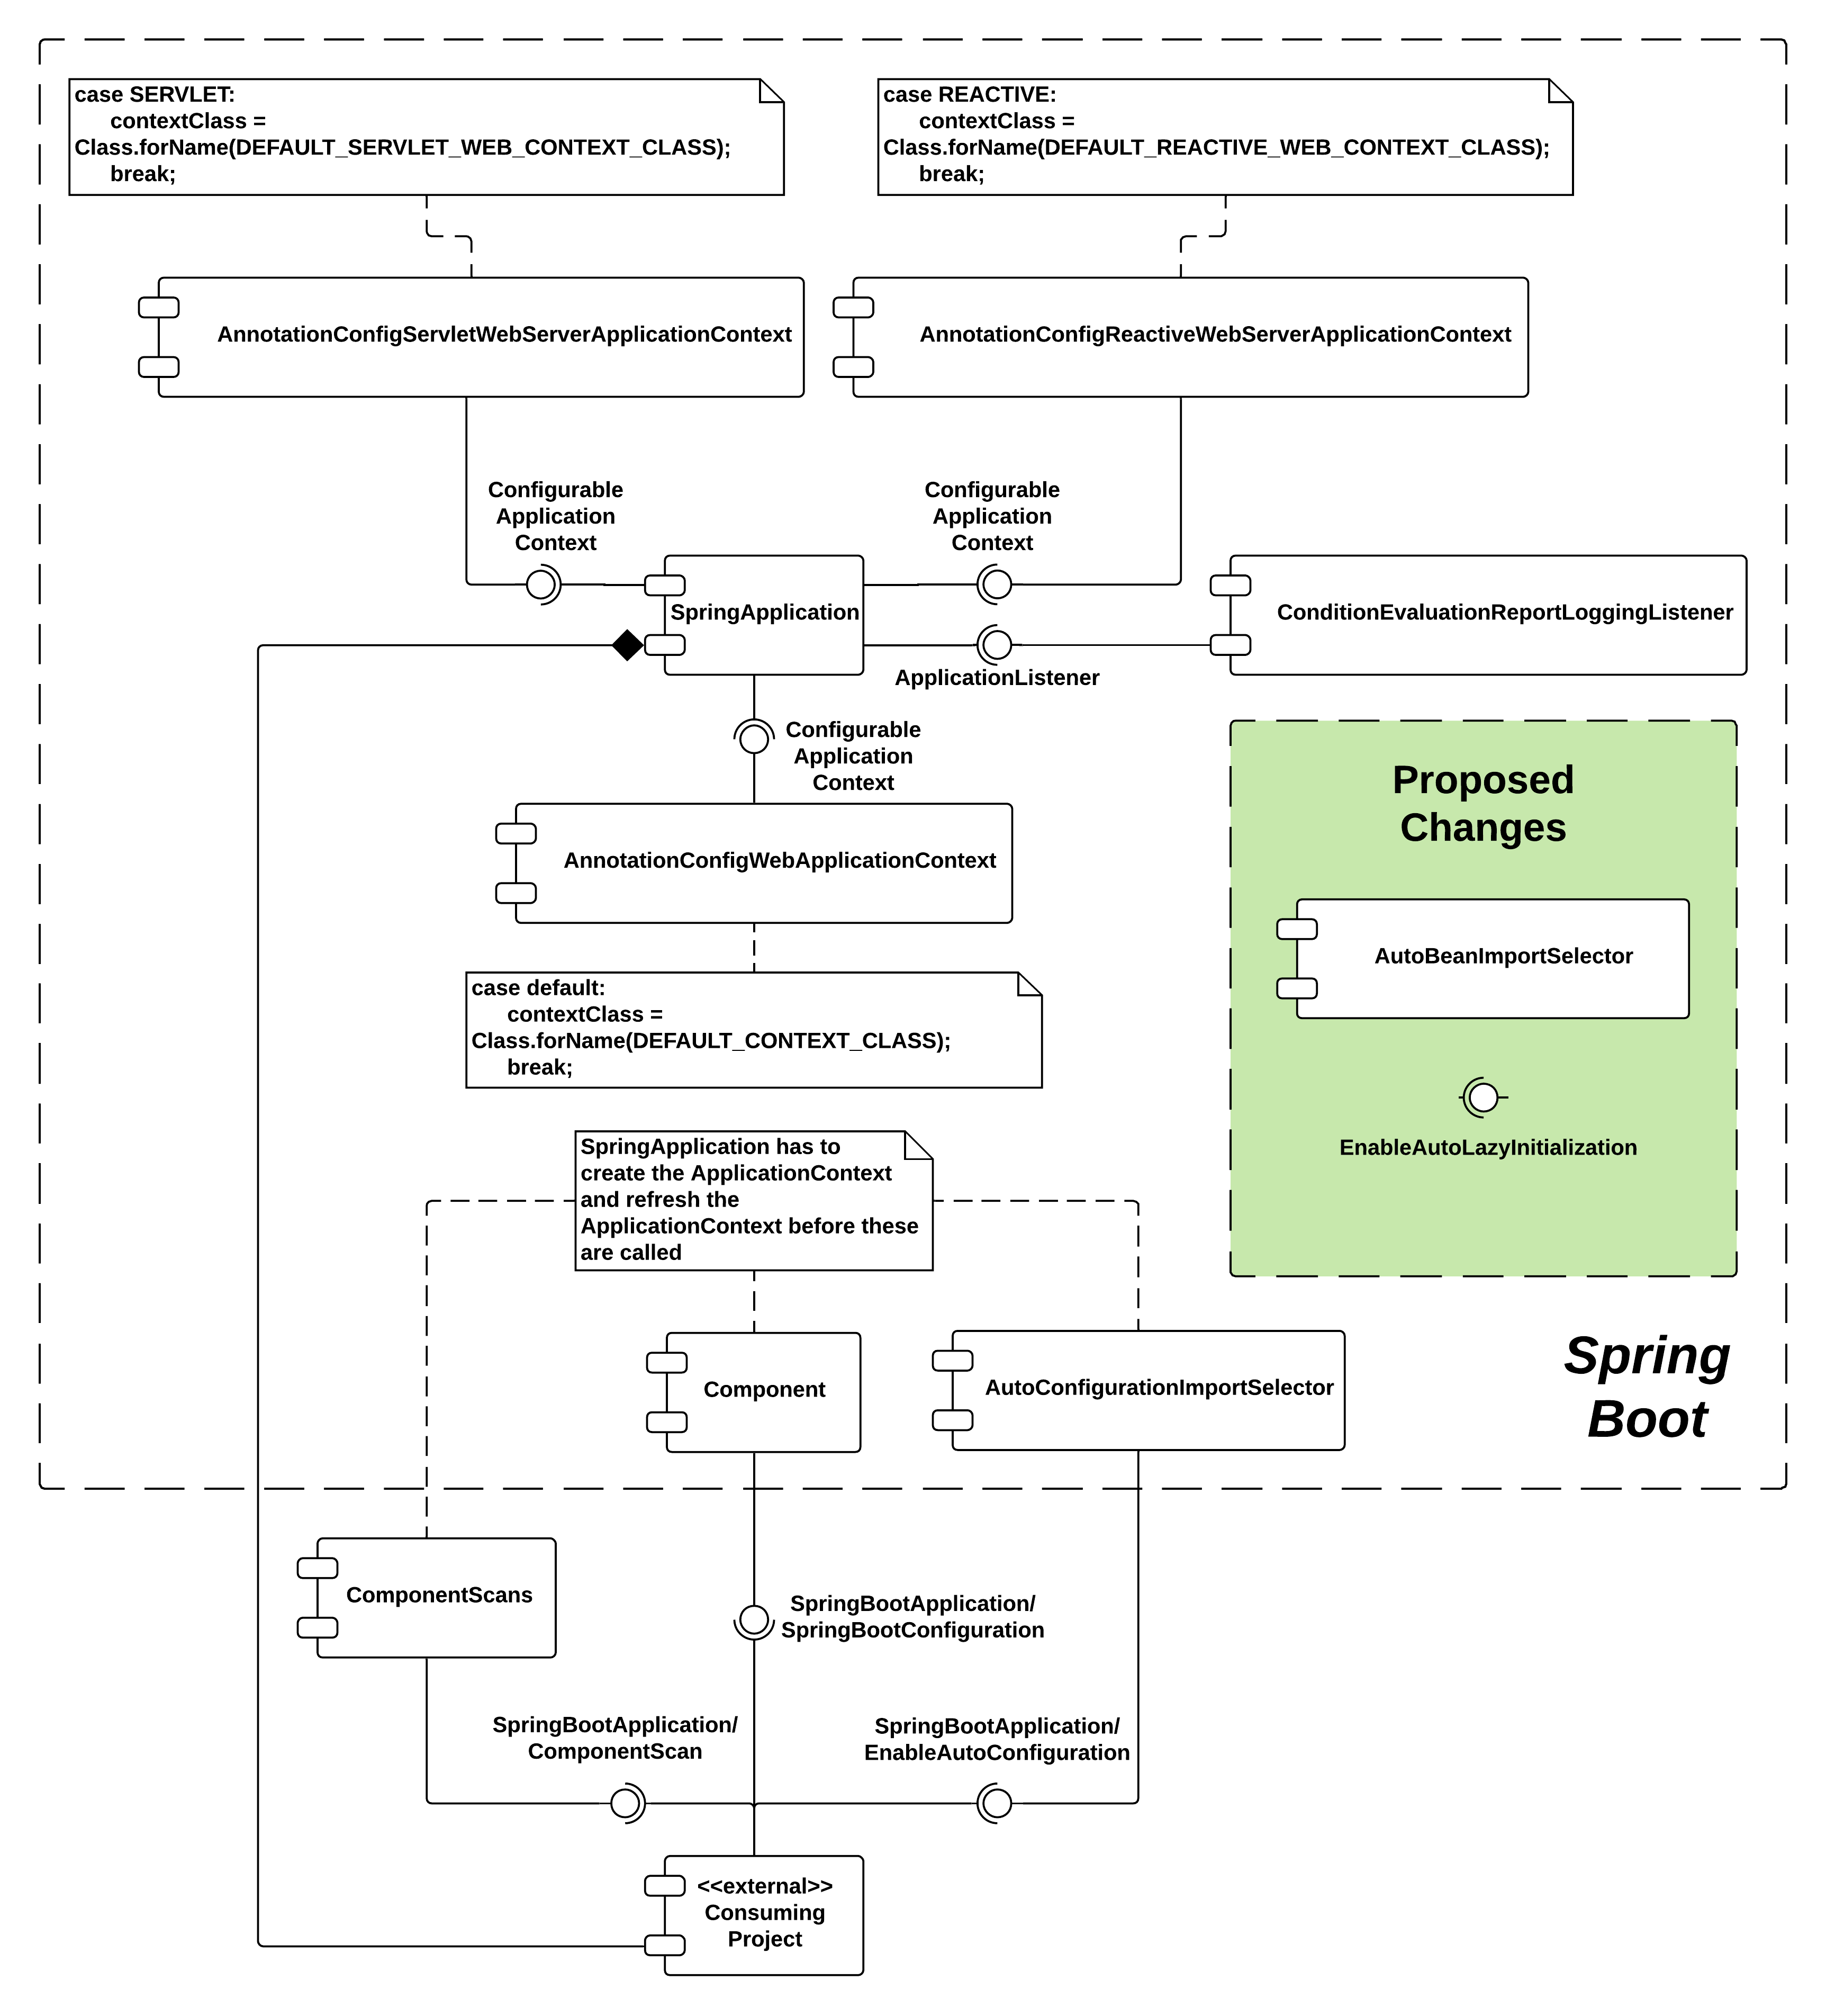
\includegraphics[width=\textwidth]{content/appendices/extension.png}
    \caption{Spring Boot Extension Proposal Diagram}
    \label{extension-diagram}
\end{figure}

